\documentclass[10pt]{article}
\usepackage[margin=1.5in]{geometry}
%%%% PACKAGES TO USE
\usepackage[utf8]{inputenc} % allow utf-8 input
\usepackage[T1]{fontenc}    % use 8-bit T1 fonts
\usepackage{hyperref}       % hyperlinks
\usepackage{url}            % simple URL typesetting
\usepackage{booktabs}       % professional-quality tables
\usepackage{amsfonts}       % blackboard math symbols
\usepackage{nicefrac}       % compact symbols for 1/2, etc.
\usepackage{microtype}      % microtypography

%% Inigo
% Math related
\usepackage{amsmath}
% Indicator
\usepackage{bbm}
% Figures and subfigures
\usepackage{graphicx}
\usepackage{caption}
\usepackage{subcaption}
% Figures stay where told
\usepackage{float}
% To draw graphs
\usepackage{tikz}
% Library for bayesian networks
\usetikzlibrary{bayesnet}
% Algorithms
\usepackage{algorithm}
\usepackage{algpseudocode} 

%%%% DEFINITIONS-MACROS: Inigo
% Real line
\def \Real{{\mathbb R}} 
\def \Natural{{\mathbb N}} 
%Expected value
\newcommand{\eValue}[1]{\mathbb{E}\left\{ #1 \right\}}
% My small matrix
\newcommand{\mySmallMatrix}[1]{\left(\begin{smallmatrix} #1 \end{smallmatrix}\right)}
% Abbreviations
\newcommand{\ie}{i.e., }
\newcommand{\Ie}{I.e., }
\newcommand{\eg}{e.g. }
\newcommand{\Eg}{E.g. }
\newcommand{\etAl}{et al.\xspace}

%% Statistical-macros
%Distributions
\newcommand{\N}{\mathcal{N}}
\newcommand{\TN}{\mathcal{TN}}
\newcommand{\G}{\mathcal{G}}
\newcommand{\T}{\mathcal{T}}
\newcommand{\U}{\mathcal{U}}
\newcommand{\Dir}{{\rm Dir}}
\newcommand{\Cat}{{\rm Cat}}
\newcommand{\Mult}{{\rm Mult}}
\newcommand{\Bin}{{\rm Bin}}
\newcommand{\IG}{{\rm IG}}
\newcommand{\NIG}{{\rm NIG}}
\newcommand{\NIX}{{\rm NIX}}
\newcommand{\IW}{{\rm IW}}
\newcommand{\NIW}{{\rm NIW}}
\newcommand{\InvGa}{{\rm IG}}
\newcommand{\Chisquare}{\Chi^2}
\newcommand{\St}{{\rm St}}
\newcommand{\Beta}{{\rm Beta}}
\newcommand{\iid}{i.i.d. }
\newcommand{\Eta}{{\cal N}}
\newcommand{\Ber}{{\rm Ber}}

%Others
\newcommand{\ind}[1]{1_{#1}} % Indicator function
\newcommand{\pr}{P} % Generic probability
\newcommand{\var}{\textrm{Var}}
\newcommand{\cov}{\textrm{Cov}}
\newcommand{\sgn}{\textrm{sgn}}
\newcommand{\sign}{\textrm{sign}}
\newcommand{\kl}{\textrm{KL}} 
\newcommand{\abs}[1]{|{#1}|}
\newcommand{\Var}{\mathrm{Var}}
\newcommand{\Cov}{\mathrm{Cov}}
\newcommand{\tr}{\mathrm{tr}}
\newcommand{\Tr}{\mathrm{Tr}}
\newcommand{\diag}{\mathrm{diag}}
\newcommand{\deq}{:=}
\newcommand{\indep}{{\;\bot\!\!\!\!\!\!\bot\;}}
\newcommand{\eps}{\varepsilon}

\newcommand{\eqd}{\stackrel{d}{=}} % equal in distribution/law/measure
\newcommand{\argmax}{\mathop{\mathrm{argmax}}}
\newcommand{\argmin}{\mathop{\mathrm{argmin}}}
\newcommand{\conv}{\textrm{conv}} % for denoting the convex hull

%%%% Title and authors
\title{Variational inference for the multi-armed contextual bandit}

\author{ I\~{n}igo Urteaga and Chris H.~Wiggins\\
	{\sf \{inigo.urteaga, chris.wiggins\}@columbia.edu} \\\\
  Department of Applied Physics and Applied Mathematics\\
	Data Science Institute\\
	Columbia University\\
	New York City, NY 10027
}

\begin{document}

\maketitle

\begin{abstract}
In many biomedical, science, and engineering problems, one must sequentially decide which action to take next so as to maximize rewards. Reinforcement learning is an area of machine learning that studies how this maximization balances exploration and exploitation, optimizing interactions with the world while simultaneously learning how the world operates. One general class of algorithms for this type of learning is the multi-armed bandit setting and, in particular, the contextual bandit case, in which observed rewards are dependent on each action as well as on given information or `context' available at each interaction with the world. The Thompson sampling algorithm has recently been shown to perform well in real-world settings and to enjoy provable optimality properties for this set of problems. It facilitates  generative and interpretable modeling of the problem at hand, though complexity of the model limits its application, since one must both sample from the distributions modeled and calculate their expected rewards. We here show how these limitations can be overcome using variational approximations, applying to the reinforcement learning case advances developed for the inference case in the machine learning community over the past two decades. We consider bandit applications where the true reward distribution is unknown and approximate it with a mixture model, whose parameters are inferred via variational inference.
\end{abstract}

\section{Introduction}
\label{sec:introduction}

The multi-armed bandit problem (\cite{b-Sutton1998,j-Ghavamzadeh2015}) is the natural abstraction for a wide variety of real-world challenges requiring learning while simultaneously maximizing reward. The goal is to decide on a series of actions under uncertainty, where each action can depend on previous rewards, actions, and contexts. Its name comes from the playing strategy one must devise when facing a row of slot machines (\ie which arms to play), and is more formally referred to as the theory of sequential decision processes. Its foundations in the field of statistics began with the work by \cite{j-Thompson1933,j-Thompson1935} and continued with the contributions by \cite{j-Robbins1952}.

Interest in sequential decision making has recently intensified in both academic and industrial communities. The publication of separate works by \cite{ic-Chapelle2011} and \cite{j-Scott2015} have shown its impact in the online content management industry. This renaissance period of the multi-armed bandit problem has both a practical aspect (\cite{j-Li2010}) and a theoretical one as well (\cite{j-Scott2010,j-Agrawal2011,ip-Maillard2011}). Interestingly, most of these works have orbited around one of the oldest heuristics that address the exploration-exploitation trade-off, \ie Thompson sampling. It has been empirically proven to perform satisfactorily and to enjoy provable optimality properties, both for problems with and without context (\cite{j-Agrawal2012,j-Agrawal2012a,ic-Korda2013,j-Russo2014,j-Russo2016}).

In this work, we are interested in extending and improving the Thompson sampling technique. Thompson sampling is applicable to restricted models of the world, as long as one can sample from the corresponding parameter posteriors and compute their expected rewards (see \cite{j-Scott2010} for details). The issue is that, for many problems of practical interest, one has partial (or no) information about the ground truth and the available models might be misspecified. We target a richer class of bandits than in the most recent literature, where the posterior is usually assumed to be from the exponential family of distributions. In this work, we aim at extending Thompson sampling to allow for more complex and flexible reward distributions. We model the convoluted relationship between the observed variables (rewards), and the unknown parameters governing the underlying process by mixture models, a large hypothesis space which for many components can accurately approximate any continuous reward distribution.

The main challenge is how to learn such a mixture distribution within the contextual multi-armed bandit setting. We leverage the advances developed for the inference case in the last decades, and propose a variational approximation to the underlying true distribution of the environment with which one interacts. Variational inference is a very principled framework, with roots in statistical physics and widely applied in the machine learning community \cite{b-Bishop2006}. The proposed method autonomously learns the parameters of the mixture model that best approximates the true underlying reward distribution.

Our contribution is unique to the bandit setting in that (a) we approximate unknown bandit reward functions with Gaussian mixture models, and (b) we provide variational mean-field parameter updates for the distribution that minimizes its divergence (in the Kullback-Leibler sense) to the mixture-model reward approximation. To the best of our knowledge, there is no other work in the literature that uses variational inference to tackle the contextual multi-armed bandit problem. The proposed algorithm is valuable when restrictive modeling assumptions are undesirable.

We formally introduce the contextual multi-armed bandit problem in Section \ref{sec:problem_formulation}, before providing a description of our proposed variational Thompson sampling method in Section \ref{sec:proposed_method}. We evaluate its performance in Section \ref{sec:evaluation}, and we conclude with final remarks in Section \ref{sec:conclusion}.

\section{Problem formulation}
\label{sec:problem_formulation}

The contextual multi-armed bandit problem is formulated as follows. Let $a\in\{1,\cdots,A\}$ be any possible action (arms in the bandit) and $f_{a}(y|x,\theta)$ the stochastic reward distribution of each arm, dependent on its properties (\ie parameters $\theta$) and context $x\in\Real^{d}$. For every time instant $t$, the observed reward $y_t$ is independently drawn from the reward distribution corresponding to the played arm, parameterized by $\theta$ and the applicable context; \ie $y_t\sim f_{a}(y|x_t,\theta)$. We denote a set of given contexts, played arms, and observed rewards up to time instant $t$ as $x_{1:t} \equiv (x_1, \cdots , x_t)$, $a_{1:t} \equiv (a_1, \cdots , a_t)$ and $y_{1:t} \equiv (y_1, \cdots , y_t)$, respectively.

In the contextual multi-armed bandit setting, one must decide which arm to play next (\ie decide $a_{t+1}$), based on the context $x_{t+1}$, and previously observed rewards $y_{1:t}$, played arms $a_{1:t}$, and contexts $x_{1:t}$. The goal is to maximize the expected (cumulative) reward. We denote each arm's expected reward as $\mu_{a}(x,\theta)=\mathbb{E}_{a}\{y|x,\theta\}$. 

When the properties of the arms (\ie their parameters) are known, one can readily determine the optimal selection policy as soon as the context is given, \ie
		\begin{equation}
		a^*(x,\theta)=\argmax_{a}\mu_{a}(x,\theta) \; .
		\end{equation}
		
The challenge in this set of problems is raised when there is a lack of knowledge about the model. The issue amounts to the need to learn about the key properties of the environment (\ie the parameters of the reward distribution), as one interacts with the world (\ie takes actions sequentially). Amongst the many alternatives to address this class of problems, the randomized probability matching is particularly appealing. In its simplest form, known as Thompson sampling, it has been shown to perform empirically well (\cite{ic-Chapelle2011, j-Scott2015}) and has sound theoretical bounds, for both contextual and context-free problems (\cite{j-Agrawal2012,j-Agrawal2012a}). This approach plays each arm in proportion to its probability of being optimal, \ie
\begin{equation}
a_{t+1} \sim \mathrm{Pr}\left[a=a_{t+1}^*|a_{1:t}, x_{1:t+1}, y_{1:t}, \theta \right] \;.
\end{equation} 

If the parameters are known, the above expression becomes deterministic, as one always picks the arm with the maximum expected reward
\begin{equation}
\begin{split}
\mathrm{Pr}\left[a=a_{t+1}^*|a_{1:t}, x_{1:t+1}, y_{1:t},\theta \right] &= \mathrm{Pr}\left[a=a_{t+1}^*|x_{t+1}, \theta \right] = I_a(x_{t+1},\theta) \;, \\
\text{with } \; I_a(x,\theta) &= \begin{cases}
1, \; \mu_{a}(x,\theta)=\max\{\mu_1(x,\theta), \cdots, \mu_A(x,\theta)\} \;, \\
0, \; \text{otherwise} \;.
\end{cases}
\label{eq:theta_known_pr_arm_optimal}
\end{split}
\end{equation}

When the parameters are unknown, one needs to explore ways of computing Eqn. \ref{eq:theta_known_pr_arm_optimal}. If we model the parameters as a set of random variables, then the uncertainty over the parameters can be accounted for. Specifically, we marginalize over their probability distribution after observing rewards and actions up to time instant $t$, \ie
\begin{equation}
\begin{split}
\mathrm{Pr}\left[a=a_{t+1}^* \big| a_{1:t}, x_{1:t+1}, y_{1:t}\right]&=\int f(a|a_{1:t}, x_{1:t+1}, y_{1:t}, \theta) f(\theta|a_{1:t}, x_{1:t}, y_{1:t}) \mathrm{d}\theta \\
	&=\int I_a(x_{t+1}, \theta) f(\theta|a_{1:t}, x_{1:t}, y_{1:t}) \mathrm{d}\theta \; .
\end{split}
\label{eq:theta_unknown_pr_arm_optimal}
\end{equation}

In a Bayesian setting, if the reward distribution is known, one would assign a prior over the parameters to compute the corresponding posterior. The analytical solution to such posteriors is available for a well known set of distributions (\cite{b-Bernardo2009}). Nevertheless, when reward distributions beyond simple well known cases (\eg Bernoulli, Gaussian, etc.) are considered, one must resort to approximations of the posterior. In this work, we leverage the variational inference methodology,
which has flourished in the inference case over the past several decades, to approximate such posteriors. 

\section{Proposed method}
\label{sec:proposed_method}

The learning process, as explained in the formulation of Section \ref{sec:problem_formulation}, requires updating the posterior of the parameters at every time instant. For computation of $f(\theta|a_{1:t}, x_{1:t}, y_{1:t})$, knowledge of the reward distribution is instrumental. Broad application of the method is typically limited by the simple distributions for which sampling and calculating expectations are feasible (\eg the exponential family).

In this work, we study finite mixture models as reward functions of the multi-armed bandit. Mixture models allow for the statistical modeling of a wide variety of stochastic phenomena; e.g., Gaussian mixture models can approximate arbitrarily well any continuous distribution and thus, provide a useful parametric framework to model unknown distributional shapes (\cite{b-McLachlan2004}). This flexibility comes at a cost, as learning the parameters of the mixture distribution becomes a challenge. In this work, we use and empirically validate variational inference to approximate underlying Gaussian mixture models in the contextual bandit case.

For the rest of the paper, we consider a mixture of $K$ Gaussian distributions per arm $a \in \{1, \cdots, A\}$, where each of the Gaussians is linearly dependent on the shared context. Formally,
\begin{equation}
f_a(y|x,\pi_{a,k}, w_{a,k}, \sigma_{a,k}^2) =\sum_{k=1}^K \pi_{a,k} \; \N(y|x^\top w_{a,k}, \sigma_{a,k}^2)  \;,
\; \text{with} \begin{cases}
\pi_{a,k}\in [0,1], \; \sum_{k=1}^K \pi_{a,k} = 1 \;,  \\
w_{a,k}\in \Real^{d} \;, \\
\sigma_{a,k}^2\in \Real^+ \;.
\end{cases}
\label{eq:gaussian_mixture_model}
\end{equation}

For our analysis, we incorporate an auxiliary mixture indicator variable $z_a$. These are 1-of-K encoded vectors, where $z_{a,k}=1$, if mixture $k$ is active; $z_{a,k}=0$, otherwise. One can now rewrite Eqn. \ref{eq:gaussian_mixture_model} as
\begin{equation}
f_a(y|x,z_{a},w_{a,k}, \sigma_{a,k}^2) =\prod_{k=1}^K \N(y|x^\top w_{a,k}, \sigma_{a,k}^2)^{z_{a,k}} \;, \quad \text{with } z_{a} \sim \Cat(\pi_{a}) \; .
\label{eq:gaussian_mixture_model_z}
\end{equation}

Since the parameters of the mixture distribution are unknown, we consider their conjugate priors
\begin{equation}
\begin{split}
f(\pi_{a}|\gamma_{a,0}) &=\Dir(\pi_a|\gamma_{a,0}) \; ,\\
f(w_{a,k}, \sigma_{a,k}^2|u_{a,k,0}, V_{a,k,0},\alpha_{a,k,0}, \beta_{a,k,0}) &= \NIG(w_{a,k}, \sigma_{a,k}^2 |u_{a,k,0}, V_{a,k,0},\alpha_{a,k,0}, \beta_{a,k,0}) \\
&= \N(w_{a,k}|u_{a,k,0}, \sigma_{a,k}^2V_{a,k,0}) \Gamma^{-1}(\sigma_{a,k}^2|\alpha_{a,k,0}, \beta_{a,k,0}). \\
\end{split}
\label{eq:mixture_model_conjugate_priors}
\end{equation}

Given a set of contexts $x_{1:t}$, played arms $a_{1:t}$, mixture assignments $z_{a,1:t}$, and observed rewards $y_{1:t}$, the joint distribution follows
\begin{equation}
\begin{split}
f(y_{1:t}, z_{a,1:t}, w_{a,k}, \sigma_{a,k}^2|a_{1:t}, x_{1:t}) = & f(y_{1:t}|a_{1:t}, x_{1:t}, z_{a,1:t}, w_{a,k}, \sigma_{a,k}^2) f(z_{a,1:t}|\pi_{a}) \\
& \; f(\pi_{a}|\gamma_{a,0}) f(w_{a,k} |u_{a,k,0},\sigma_{a,k}^2, V_{a,k,0}) f(\sigma_{a,k}^2|\alpha_{a,k,0}, \beta_{a,k,0})\;,
\end{split}
\end{equation}
with 
\begin{equation}
\begin{split}
f(y_{1:t}|a_{1:t}, x_{1:t}, z_{a,1:t}, w_{a,k}, \sigma_{a,k}^2) &= \prod_{t} \prod_k \N(y_t|x_t^\top w_{a,k}, \sigma_{a,k}^2)^{z_{a,k,t}} \;,\\
f(z_{1:t}|a_{1:t},\pi_a) &= \prod_t \prod_k \pi_{a,k}^{z_{a,k,t}} \;,
\end{split}
\end{equation}
and parameter priors as in Eqn. \ref{eq:mixture_model_conjugate_priors}.

\subsection{Variational approximation to the parameter posterior}
\label{ssec:variational_distribution}

For the model as described above, the true joint posterior distribution is intractable. Under the variational framework, we consider instead a restricted family of distributions and find the one that is a locally optimal approximation to the full posterior.

We do so by minimizing the Kullback-Leibler divergence between the true distribution $f(\cdot)$, and our approximating distribution $q(\cdot)$. We 
here consider
%study 
a set of parameterized distributions with the following mean-field factorization over the variables of interest
\begin{equation}
q(Z, \pi, w, \sigma^2)=q(Z) \prod_{a=1}^A q(\pi_a) \prod_{k=1}^{K} q(w_{a,k}, \sigma_{a,k}^2) \; ,
\label{eq:variational_factorization}
\end{equation}
where we introduce notation 
  $Z=\{z_{a,k,t}\}, \forall a,k,t$; 
  $\pi=\{\pi_{a,k}\}, \forall a,k$; 
  $w=\{w_{a,k}\}, \forall a,k$; 
  and 
  $\sigma^2=\{\sigma_{a,k}^2\}, \forall a,k$. 
We place no restriction on the functional form of each distributional factor, and we seek to optimize the Kullback-Leibler divergence between this and the true distribution.

We illustrate the graphical model of the true and the variational bandit distributions in Fig. \ref{fig:graphical_bandit}.

% Bandit graphical Models
\begin{figure}[h]
	\centering
	\begin{subfigure}[b]{0.49\textwidth}
		\begin{center}
			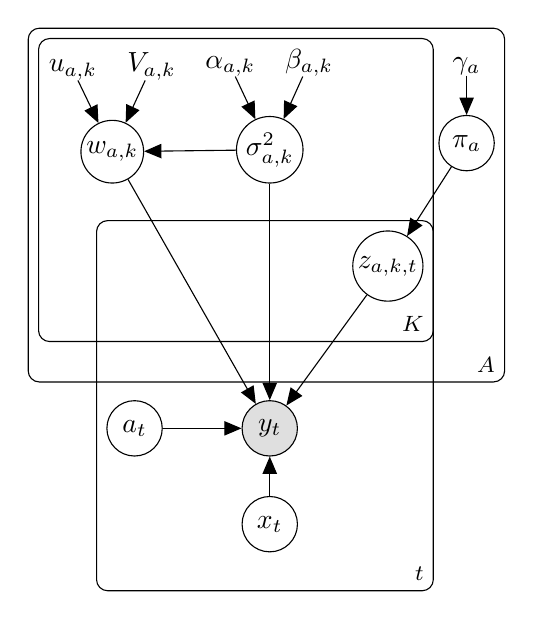
\begin{tikzpicture}
	% Nodes
	% Return y
	\node[obs] (y-t) {$y_{t}$};
	% Linear Gaussian parameters
	\node[latent, above=2.75 of y-t, xshift=-2cm]  (w-ak) {$w_{a,k}$};
	\node[latent, above=2.75 of y-t, xshift=0cm] (sigma-ak) {$\sigma_{a,k}^2$};
	% Mixture indicator z
	\node[latent, above=1.25 of y-t, xshift=1.5cm] (z-akt) {$z_{a,k,t}$};
	% Mixture proportions pi
	\node[latent, above=0.75 of z-akt, xshift=1cm] (pi-a) {$\pi_{a}$};	
	% Action a
	\node[latent, left=1 of y-t] (a-t) {$a_t$};
	% Context x
	\node[latent, below=0.5 of y-t]  (x-t) {$x_t$};
	
	% Hyperparameters: constants
	% \sigma's IG hyperparameters
	\node[const, above=0.5 of sigma-ak, xshift=-0.5cm] (alpha-ak) {$\alpha_{a,k}$} ;
	\node[const, above=0.5 of sigma-ak, xshift=0.5cm]  (beta-ak) {$\beta_{a,k}$} ;
	
	% \theta' N hyperparameters
	\node[const, above=0.5 of w-ak, xshift=-0.5cm] (mu-ak) {$u_{a,k}$} ;
	\node[const, above=0.5 of w-ak, xshift=0.5cm]  (V-ak) {$V_{a,k}$} ;
	
	% pi's Dirichlet hyperparameters
	\node[const, above=0.5 of pi-a] (gamma-a) {$\gamma_{a}$} ;
	
	% Edges
	% Connect sigma hyperparameters
	\edge {alpha-ak,beta-ak} {sigma-ak} ;
	% Connect theta hyperparameters
	\edge {mu-ak,V-ak,sigma-ak} {w-ak} ;
	% Connect mixture proportion hyperparameters
	\edge {gamma-a} {pi-a} ;
	% Connect mixture proportions to indicators
	\edge {pi-a} {z-akt} ;
	% Connect mixture parameters, mixture indicator, context and arm to observation
	\edge {sigma-ak, w-ak, z-akt,x-t,a-t} {y-t} ;
	
	% Plates
	% Over time
	\plate {t} {(a-t)(x-t)(z-akt)(y-t)} {$t$} ;
	% Over each mixture
	\plate {k}{
		(alpha-ak)(beta-ak)(mu-ak)(V-ak) % hyperparameters
		(sigma-ak)(w-ak) % parameters
		(z-akt) % indicator
		} {$K$} ;
	% Over each arm
	\plate {a}{
		(alpha-ak)(beta-ak)(mu-ak)(V-ak)(gamma-a) % hyperparameters
		(sigma-ak)(w-ak)(pi-a) % parameters
		(z-akt) % indicator
		(k.north west) (k.south west) % Extra space
	} {$A$} ;
\end{tikzpicture}
		\end{center}
		\label{fig:true_bandit}
		\caption{True contextual bandit distribution.}
	\end{subfigure}
	%add desired spacing between images, e. g. ~, \quad, \qquad etc.
	%(or a blank line to force the subfigure onto a new line)
	\begin{subfigure}[b]{0.49\textwidth}	
		\begin{center}
			%\begin{tikzpicture}[x=1.7cm,y=1.8cm]
\begin{tikzpicture}
	% Nodes
	% Return y
	\node[obs] (y-t) {$y_{t}$};
	% Linear Gaussian parameters
	\node[latent, above=2.75 of y-t, xshift=-2cm]  (w-ak) {$w_{a,k}$};
	\node[latent, above=2.75 of y-t, xshift=0cm] (sigma-ak) {$\sigma_{a,k}^2$};
	% Mixture indicator z
	\node[latent, above=0.75 of y-t, xshift=1.5cm] (z-akt) {$z_{a,k,t}$};
	% Mixture proportions pi
	\node[latent, above=1.25 of z-akt, xshift=1cm] (pi-a) {$\pi_{a}$};	
	% Action a
	\node[latent, left=1 of y-t] (a-t) {$a_t$};
	% Context x
	\node[latent, below=0.5 of y-t]  (x-t) {$x_t$};
	
	% Hyperparameters: constants
	% \sigma's IG hyperparameters
	\node[const, above=0.5 of sigma-ak, xshift=-0.5cm] (tildealpha-ak) {$\widetilde{\alpha}_{a,k}$} ;
	\node[const, above=0.5 of sigma-ak, xshift=0.5cm]  (tildebeta-ak) {$\widetilde{\beta}_{a,k}$} ;
	
	% \theta' N hyperparameters
	\node[const, above=0.5 of w-ak, xshift=-0.5cm] (tildew-ak) {$\widetilde{u}_{a,k}$} ;
	\node[const, above=0.5 of w-ak, xshift=0.5cm]  (tildeV-ak) {$\widetilde{V}_{a,k}$} ;
	
	% pi's Dirichlet hyperparameters
	\node[const, above=0.5 of pi-a] (tildegamma-ak) {$\widetilde{\gamma}_{a,k}$} ;

	% z's multinomial hyperparameters
	\node[const, above=0.5 of z-akt] (r-akt) {$r_{a,k,t}$} ;
	
	% Edges
	% Connect sigma hyperparameters
	\edge {tildealpha-ak,tildebeta-ak} {sigma-ak} ;
	% Connect theta hyperparameters
	\edge {tildew-ak,tildeV-ak,sigma-ak} {w-ak} ;
	% Connect mixture proportion hyperparameters
	\edge {tildegamma-ak} {pi-a} ;
	% Connect mixture parameters, mixture indicator, context and arm to observation
	\edge {sigma-ak, w-ak, z-akt,x-t,a-t} {y-t} ;
	% Connect mixture parameters to indicators
	\edge {r-akt} {z-akt} ;
	
	% Plates
	% Over time
	\plate {t} {(a-t)(x-t)(z-akt)(y-t)(r-akt)} {$t$} ;
	% Over each mixture and arm
	\plate {k}{
		(tildealpha-ak)(tildebeta-ak)(tildew-ak)(tildeV-ak)(tildegamma-ak) % hyperparameters
		(sigma-ak)(w-ak) % parameters
		(z-akt)(r-akt) % indicator
		} {$K$,$A$} ;
\end{tikzpicture}
		\end{center}
		\label{fig:variational_bandit}
		\caption{Variational contextual bandit distribution.}
	\end{subfigure}
	\caption{Graphical models of the bandit distribution.}
	\label{fig:graphical_bandit}
\end{figure}

The optimal solution for each variational factor in the distribution in Eqn. \ref{eq:variational_factorization} is obtained by computing the expectation of the log-joint true distribution with respect to the rest of the variational factor distributions (\cite{b-Bishop2006}).

In our setting, we compute
\begin{equation}
\begin{cases}
\ln q(Z) =\eValue{\ln\left[f(y_{1:t}, Z, w, \sigma|a_{1:t}, x_{1:t})\right]}_{\pi, w, \sigma}+c \;, \\
\ln q(\pi_a) =\eValue{\ln\left[f(y_{1:t}, Z, w, \sigma|a_{1:t}, x_{1:t})\right]}_{Z, w, \sigma}+c \;,\\
\ln q(w_{a,k},\sigma_{a,k}^2) =\eValue{\ln\left[f(y_{1:t}, Z, w, \sigma|a_{1:t}, x_{1:t})\right]}_{Z,\pi}+c \;.\\
\end{cases}
\end{equation}

The resulting solution to the variational parameters that minimize the divergence of our approximation iterates over the following two steps:
\begin{enumerate}
	\item Given the current variational parameters, compute the responsibilities
		\begin{equation}
		\begin{split}
		\log (r_{a,k,t}) &= -\frac{1}{2} \left[\ln\left(\widetilde{\beta}_{a,k}\right) - \psi \left(\widetilde{\alpha}_{a,k}\right)\right] -\frac{1}{2} \left[x_t^\top \widetilde{V}_{a,k} x_t + (y_t-x_t^\top \widetilde{u}_{a,k})^2\frac{\widetilde{\alpha}_{a,k}}{\widetilde{\beta}_{a,k}}\right] \\
		& \qquad + \left[\psi(\widetilde{\gamma}_{a,k})- \psi\left(\sum_{k=1}^K\widetilde{\gamma}_{a,k}\right)\right] + c \;,
		\end{split}
		\end{equation}
		with $\sum_{k=1}^K r_{a,k,t} = 1$. These responsibilities correspond to the expected value of assignments, \ie $r_{a,k,t}=\eValue{z_{a,k,t}}_{Z}$.
	\item Given the current responsibilities, we define $R_{a,k}\in\Real^{t\times t}$ as a sparse diagonal matrix with diagonal elements $\left[R_{a,k}\right]_{t,t^\prime}=r_{a,k,t} \cdot \mathbbm{1}[a_t=a]$, and update the variational parameters
		\begin{equation}
		\begin{cases}
		\widetilde{\gamma}_{a,k}=\gamma_{a,0} + \tr\{R_{a,k}\} \;, \\
		\widetilde{V}_{a,k}^{-1} = x_{1:t} R_{a,k} x_{1:t}^\top + V_{a,k,0}^{-1} \;,\\
		\widetilde{u}_{a,k}= \widetilde{V}_{a,k} \left( x_{1:t} R_{a,k} y_{1:t} + V_{a,k,0}^{-1} u_{a,k,0}\right) \;, \\
		\widetilde{\alpha}_{a,k} = \alpha_{a,k,0} + \frac{1}{2} \tr\{R_{a,k}\} \;, \\
		\widetilde{\beta}_{a,k} = \beta_{a,k,0} + \frac{1}{2}\left(y_{1:t}^\top R_{a,k}y_{1:t} + u_{a,k,0}^\top V_{a,k,0}^{-1} u_{a,k,0} - \widetilde{u}_{a,k}^\top \widetilde{V}_{a,k}^{-1} \widetilde{u}_{a,k} \right) \; .\\
		\end{cases}
		\end{equation}
\end{enumerate}

The above iterative process is repeated until a convergence criterion is met. Usually, one iterates until the optimization improvement is small (relative to some prespecified $\epsilon$) or a maximum number of iterations is met.

Note that we have considered the same number of mixtures per arm $K$, but the above expressions are readily 
%applicable 
generalizable
to differing per-arm number of mixtures $K_a$, for $a\in\{1, \cdots, A\}$.

\subsection{Variational Thompson sampling}
\label{ssec:variational_thompson_sampling}

We now describe our proposed variational Thompson sampling (VTS) technique for the multi-armed contextual bandit problem, which leverages the variational distribution in subsection \ref{ssec:variational_distribution} and implements a sampling based policy.

In the multi-armed bandit, at any given time instant and based on the information available, one needs to decide which arm to play next. A randomized probability matching technique picks the arm that has the highest probability of being optimal. In its simplest form, known as Thompson sampling (\cite{j-Thompson1935}), instead of computing the integral in Eqn. \ref{eq:theta_unknown_pr_arm_optimal}, one draws a random parameter sample from the posterior and then picks the action that maximizes the expected reward. That is, 
\begin{equation}
a_{t+1}=\argmax_{a}\mu_{a}(x_{t+1},\theta_{t+1}), \; \text{ with } \; \theta_{t+1} \sim f(\theta|a_{1:t}, x_{1:t}, y_{1:t}) \; .
\end{equation}
In a pure Bayesian setting, one deals with simple models that allow for analytical computation (and sampling) of the posterior. Here, as we allow for more realistic and complex modeling of the world that may not result in closed-form posterior updates, we propose to sample the parameters from the variational approximating distributions computed in subsection \ref{ssec:variational_distribution}.

We describe the proposed variational Thompson sampling technique in Algorithm \ref{alg:vts} (expressed for a general Gaussian mixture model with context).

%VTS
\begin{algorithm}
	\begin{algorithmic}
	\Require $A$, $K_a$ and parameters $\gamma_{a,0}$, $u_{a,k,0}$, $V_{a,k,0}$, $\alpha_{a,k,0}$, $\beta_{a,k,0}$
	\State $D=\emptyset$
	\State Initialize $\widetilde{\gamma}_{a,k}=\gamma_{a,0}, \widetilde{\alpha}_{a,k}=\alpha_{a,k,0}, \widetilde{\beta}_{a,k}=\beta_{a,k,0}, \widetilde{u}_{a,k}=u_{a,k,0}, \widetilde{V}_{a,k}=V_{a,k,0}$
	\For{$t=1, \cdots, T$}
		\State Receive context $x_{t+1}$
		\For{$a=1, \cdots, A$}
			\For{$k=1, \cdots, K_a$}
				\State Draw $\theta_{a,k,t+1} \sim q\left(\widetilde{\gamma}_{a,k}, \widetilde{\alpha}_{a,k}, \widetilde{\beta}_{a,k}, \widetilde{u}_{a,k}, \widetilde{V}_{a,k}\right)$
			\EndFor
			\State Compute $\mu_{a,t+1}=\mu_{a}(x_{t+1},\theta_{a,t+1})$
		\EndFor
		\State Play arm $a_{t+1}=\argmax_{a}\mu_{a,t+1}$
		\State Observe reward $y_{t+1}$
		\State $D=D \cup \left\{x_{t+1}, a_{t+1}, y_{t+1}\right\}$
		\While{Variational convergence criteria not met}
			\State Compute $r_{a,k,t}$
			\State Update $\widetilde{\gamma}_{a,k}, \widetilde{\alpha}_{a,k}, \widetilde{\beta}_{a,k}, \widetilde{u}_{a,k}, \widetilde{V}_{a,k}$
		\EndWhile
	\EndFor
	\end{algorithmic}
	\caption{Variational Thompson sampling}
	\label{alg:vts}
\end{algorithm}

An instrumental step in the proposed algorithm is to compute the expected reward for each arm, \ie $\mu_{a,t+1}$. Since we are dealing with mixture models, the following approaches can be considered:
\begin{enumerate}
	\item Expectation with mixture assignment sampling
	\begin{equation}
	\mu_{a,t+1}=x_{t}^\top \widetilde{u}_{a,z_{a,k,t}} \;, \qquad \text{ with } \; z_{a,k,t} \sim \Cat \left(\frac{\widetilde{\gamma}_{a,k}}{\sum_{k=1}^{K}\widetilde{\gamma}_{a,k}} \right) \;.
	\end{equation}
	\item Expectation with mixture proportion sampling
	\begin{equation}
	\mu_{a,t+1}=\sum_{k=1}^K \pi_{a,k,t} x_{t}^\top \widetilde{u}_{a,k} \;, \qquad \text{ with } \; \pi_{a,k,t} \sim \Dir\left(\widetilde{\gamma}_{a,k} \right) \;.
	\end{equation}
	\item Expectation with mixture proportions
	\begin{equation}
	\mu_{a,t+1}=\sum_{k=1}^K \pi_{a,k,t} x_{t}^\top \widetilde{u}_{a,k} \;, \qquad \text{ with } \; \pi_{a,k,t} = \frac{\widetilde{\gamma}_{a,k}}{\sum_{k=1}^{K}\widetilde{\gamma}_{a,k}} \;.
	\end{equation}
\end{enumerate}

\section{Evaluation}
\label{sec:evaluation}

In this section, we evaluate the performance of the proposed variational Thompson sampling technique for the contextual multi-armed bandit problem. We consider the two-armed contextual linear Gaussian bandit, with a two dimensional uncorrelated uniform context $x_{i,t}\sim\U(0,1)$, $i\in\{1,2\}$, $t\in \Natural$.

We focus on two illustrative scenarios: the first, referred to as \texttt{Scenario A}, with per-arm reward distributions
\begin{equation}
\texttt{Scenario A }\begin{cases}
f_{0}(y|x_t,\theta) = 0.5 \cdot \N\left(y|(0 \; 0)^\top x_t , 1\right) + 0.5 \cdot \N\left(y|(1 \; 1)^\top x_t , 1\right) \; ,\\
f_{1}(y|x_t,\theta) = 0.5 \cdot \N\left(y|(2 \; 2)^\top x_t , 1\right) + 0.5 \cdot \N\left(y|(3 \; 3)^\top x_t , 1\right) \; ,
\end{cases}
\label{eq:scenario_A}
\end{equation}
and the second, \texttt{Scenario B}, with
\begin{equation}
\texttt{Scenario B }\begin{cases}
f_{0}(y|x_t,\theta) = 0.5 \cdot \N\left(y|(1 \; 1)^\top x_t , 1\right) + 0.5 \cdot \N\left(y|(2 \; 2)^\top x_t , 1\right) \; ,\\
f_{1}(y|x_t,\theta) = 0.3 \cdot \N\left(y|(0 \; 0)^\top x_t , 1\right) + 0.7 \cdot \N\left(y|(3 \; 3)^\top x_t , 1\right) \; .
\end{cases}
\label{eq:scenario_B}
\end{equation}
The per-arm reward distributions of the contextual bandits in both scenarios are Gaussian mixtures with two context dependent components. However, the amount of mixture overlap and the similarity between arms differ. Recall the complexity of the reward distributions in \texttt{Scenario B}, with a significant overlap between the arms and the unbalanced nature of arm 1.

Fig. \ref{fig:cumregret_comparison} shows the cumulative regret of the proposed variational Thompson sampling approach in both scenarios, when different assumptions for the variational approximating distribution are made (\ie assumed prior $K$). We define the cumulative regret as
\begin{equation}
R_t=\sum_{\tau=0}^t \eValue{\left(y^*_{\tau}-y_{\tau} \right)} = \sum_{\tau=0}^t \mu_\tau^*-\bar{y}_{\tau} \; ,
\end{equation}
where for each time instant $t$, $\mu_t^*$ denotes the expected reward of the optimal arm, and $\bar{y}_{t}$ the empirical mean of the observed rewards. Reported values are averages over 2000 realizations of the same set of parameters and context (with the standard deviation shown as the shaded region).

Since we have not observed significant cumulative regret differences between the three approaches to computing the expected reward $\mu_{a,t+1}$ described in subsection \ref{ssec:variational_thompson_sampling}, we avoid unnecessary clutter and do not plot them in Fig. \ref{fig:cumregret_comparison}.

Note that ``\textit{VTS with }$K=1$'' is equivalent to a vanilla Thompson sampling approach with a linear contextual Gaussian model assumption. Since $r_{a,k=1,t}=1$ for all $a$ and $t$, the variational update equations match the corresponding Bayesian posterior updates for Thompson sampling. We are thus effectively comparing the performance of the proposed method to the Thompson sampling benchmark.

% Cumulative regret
\begin{figure}[!h]
	\centering
	\begin{subfigure}[b]{0.48\textwidth}
		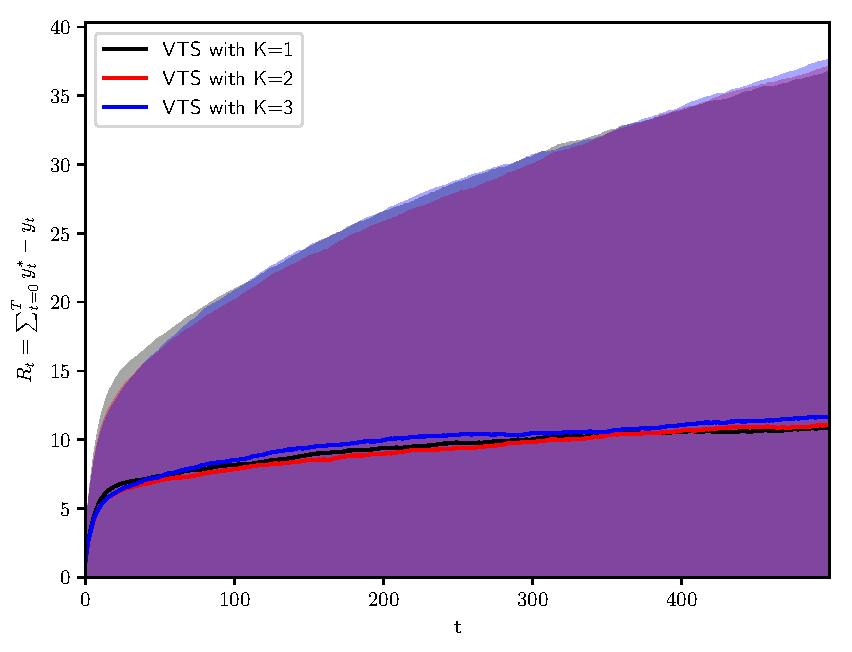
\includegraphics[width=\textwidth]{./figs/model_a_cumregret.pdf}
		\caption{\texttt{Scenario A}: cumulative regret.}
		\label{fig:model_a_cumregret}
	\end{subfigure}
	\begin{subfigure}[b]{0.49\textwidth}
		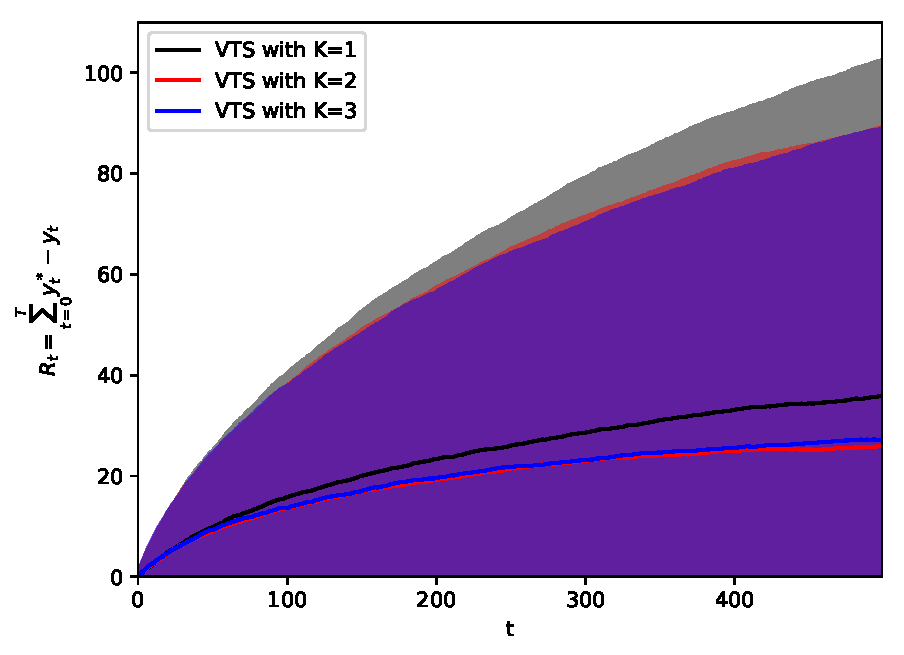
\includegraphics[width=\textwidth]{./figs/model_b_cumregret.pdf}
		\caption{\texttt{Scenario B} cumulative regret.}
		\label{fig:model_b_cumregret}
	\end{subfigure}%
	\caption{Cumulative regret comparison.}
	\label{fig:cumregret_comparison}
\end{figure}

The main conclusion from the results shown in Fig. \ref{fig:cumregret_comparison} is that inferring a variational approximation to the true complex reward distribution improves regret performance. For both scenarios, the best performance is achieved when the assumed $K$s match the true number of mixtures per arm (\texttt{Scenario A} and \texttt{Scenario B} are both a mixture of two Gaussians). As in any posterior sampling algorithm, the cumulative regret variability is large, but we observe a reduced regret variability for the proposed ``\textit{VTS with }$K=2$ and $K=3$'', in comparison to the contextual linear Gaussian Thompson sampling (\ie ``\textit{VTS with }$K=1$'').

It is interesting to observe that, for \texttt{Scenario A}, ``\textit{VTS with }$K=1$'' performs reasonably well. On the contrary, for \texttt{Scenario B}, such an assumption results in higher regret. In other words, a misspecified model performs worse than the proposed alternatives. Specially, in comparison with ``\textit{VTS with }$K=2$'', which corresponds to the true underlying mixture distributions in Eqns. \ref{eq:scenario_A} and \ref{eq:scenario_B}. Precisely, the cumulative regret reduction of ``\textit{VTS with }$K=2$'' with respect to ``\textit{VTS with }$K=1$'' at $t=500$ is of 14\% for \texttt{Scenario A} and 28\% for \texttt{Scenario B}.
The issue of model misspecification is more evident for \texttt{Scenario B}, as the linear Gaussian contextual model fails to capture the subtleties of the unbalanced mixtures of Eqn. \ref{eq:scenario_B}.

In summary, with a simplistic model assumption as in ``\textit{VTS with }$K=1$'', one can not capture the properties of the underlying reward distribution and thus, can not make well-informed decisions. However, by allowing for more complex modeling (\ie Gaussian mixture models) and by using variational inference for learning its parameters, the proposed technique attains reduced regret for both studied models.

Furthermore, we highlight that even an overly complex model assumption does provide competitive performance. For both \texttt{Scenario A} and \texttt{B}, the regret of the variational approximation with $K=3$ is similar to that of the true model assumption $K=2$, (``\textit{VTS with }$K=3$'' and ``\textit{VTS with }$K=2$'' in Fig. \ref{fig:cumregret_comparison}, respectively). The explanation relies on the flexibility provided by the variational machinery, as the learning process adjusts the parameters to minimize the divergence between the true and the variational distributions. Nonetheless, one must be aware that this flexibility comes with an additional computational cost, as more parameters need to be learned.

We further elaborate on the analysis of our proposed method by studying its learning accuracy. In bandit algorithms, the goal is to gather enough evidence to identify the best arm, and this can only be achieved if the learning of the arm properties is accurate.

We illustrate in Fig. \ref{fig:mse_comparison} the mean squared error of the per-arm expected reward
\begin{equation}
MSE_a=\frac{1}{T}\sum_{t=0}^T \left(\mu_{a,t}-\hat{\mu}_{a,t} \right)^2 \; ,
\end{equation}
where $\hat{\mu}_{a,t}$ denotes the estimated expected reward for arm $a$ at time $t$.

% MSE results (moved here for better placement)
\begin{figure}[!h]
	\centering
	\begin{subfigure}[b]{0.48\textwidth}
		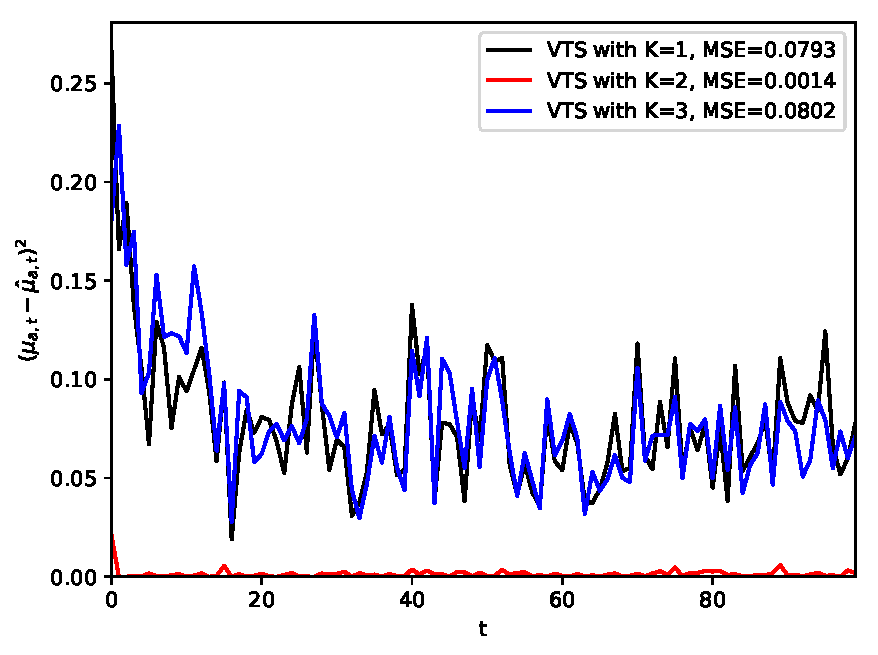
\includegraphics[width=\textwidth]{./figs/model_a_mse_arm_0.pdf}
		\caption{MSE for \texttt{Scenario A}, arm 0.}
		\label{fig:model_a_mse_arm_0}
	\end{subfigure}
	%add desired spacing between images, e. g. ~, \quad, \qquad etc.
	%(or a blank line to force the subfigure onto a new line)
	\begin{subfigure}[b]{0.46\textwidth}
		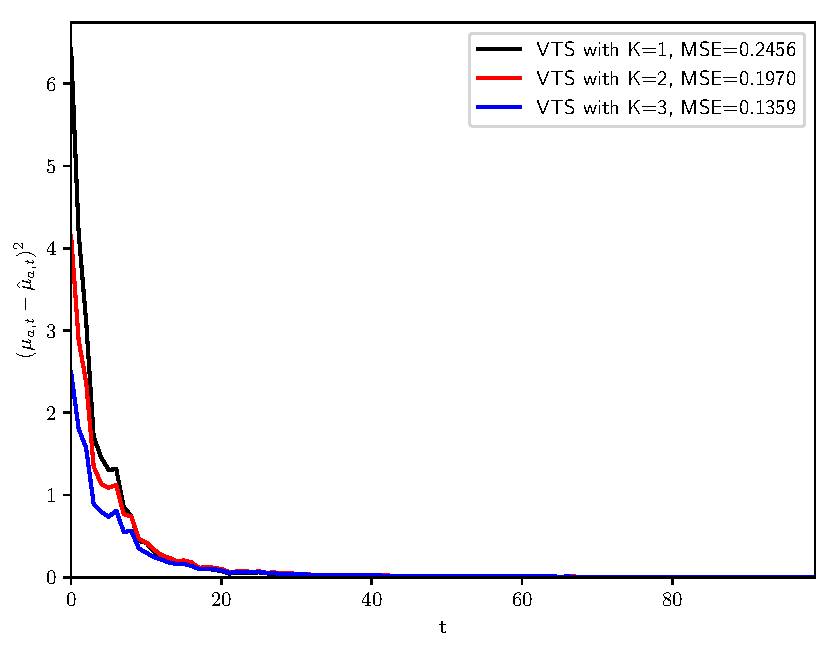
\includegraphics[width=\textwidth]{./figs/model_a_mse_arm_1.pdf}
		\caption{MSE for \texttt{Scenario A}, arm 1.}
		\label{fig:model_a_mse_arm_1}
	\end{subfigure}
	
	\begin{subfigure}[b]{0.48\textwidth}
		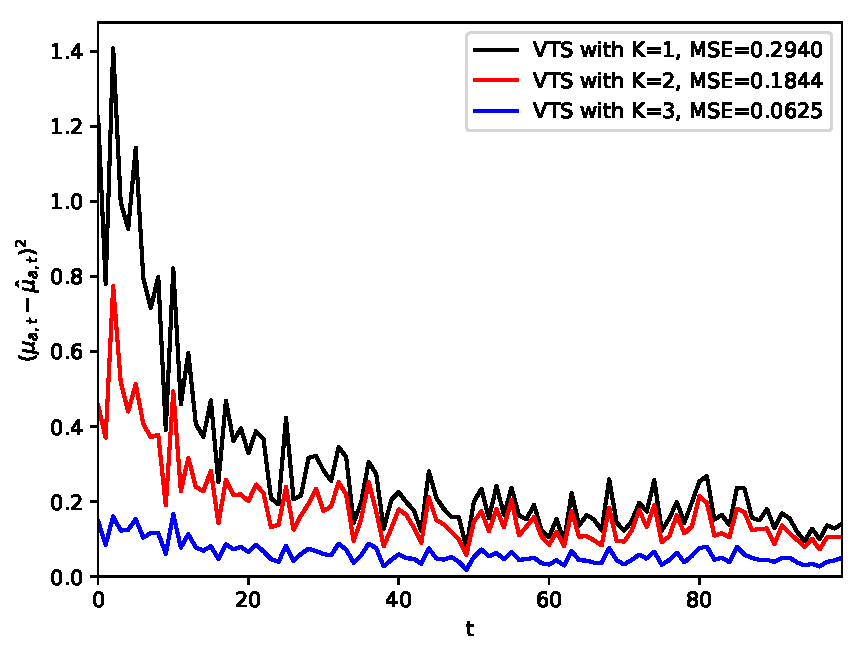
\includegraphics[width=\textwidth]{./figs/model_b_mse_arm_0.pdf}
		\caption{MSE for \texttt{Scenario B}, arm 0.}
		\label{fig:model_b_mse_arm_0}
	\end{subfigure}
	\begin{subfigure}[b]{0.48\textwidth}
		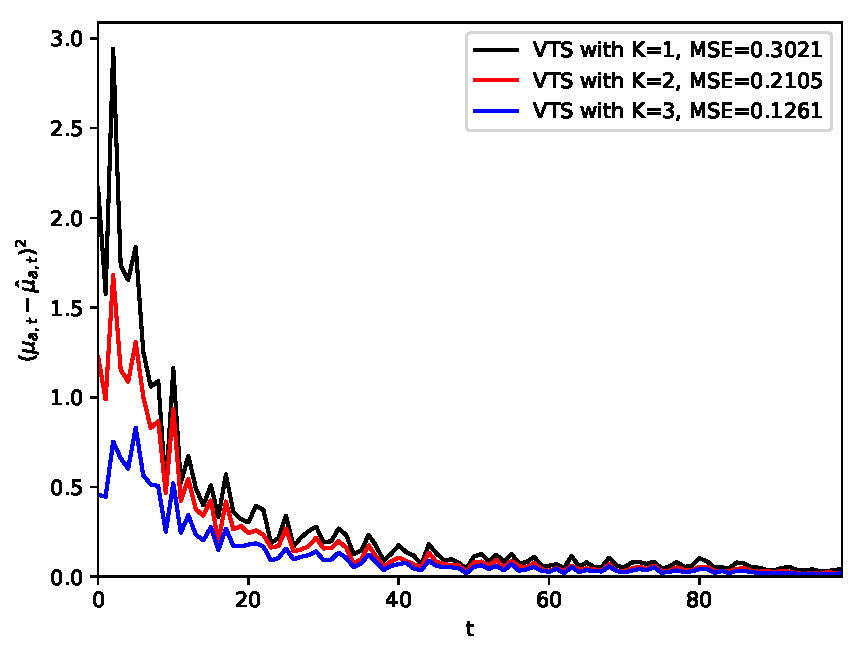
\includegraphics[width=\textwidth]{./figs/model_b_mse_arm_1.pdf}
		\caption{MSE for \texttt{Scenario B}, arm 1.}
		\label{fig:model_b_mse_arm_1}
	\end{subfigure}
	\caption{Expected reward estimation accuracy comparison.}
	\label{fig:mse_comparison}
\end{figure}

We show that the learning is faster and more accurate when the approximating mixture model has flexibility to adapt. That is, both ``\textit{VTS with }$K=2$ and ``\textit{VTS with }$K=3$ can accurately estimate the expected reward of the best arm.

We emphasize the additional complexity of \texttt{Scenario B} in comparison to \texttt{Scenario A}, and its implications. In Figs. \ref{fig:model_a_mse_arm_0}-\ref{fig:model_a_mse_arm_1}, the simplest model that assumes a single Gaussian distribution (``\textit{VTS with }$K=1$'') is able to quickly and accurately estimate the expected reward. In contrast, its estimation accuracy is the worst when facing a more complex model (as shown in Figs. \ref{fig:model_b_mse_arm_0}-\ref{fig:model_b_mse_arm_1}). Note how for all results in Fig. \ref{fig:mse_comparison}, the most complex model (\ie ``\textit{VTS with }$K=3$'') fits the expected reward best.

These observations reinforce our claims on the flexibility of the presented technique. By allowing for complex modeling of the world and using variational inference to learn it, the proposed variational Thompson sampling can provide improved performance (in the sense of regret) for the contextual multi-armed bandit problem.

%\subsubsection*{Acknowledgments}
%
%Use unnumbered third level headings for the acknowledgments. All
%acknowledgments go at the end of the paper. Do not include
%acknowledgments in the anonymized submission, only in the final paper.

\section{Conclusion}
\label{sec:conclusion}

We have presented Variational Thompson Sampling, a new algorithm for the contextual multi-armed bandit setting, where we combine the variational inference machinery with a state of the art reinforcement learning technique. The proposed variational Thompson sampling allows for interpretable bandit modeling with complex reward functions learned from online data, extending the applicability of Thompson sampling by accommodating more realistic and complex models of the world. Empirical results show a significant cumulative regret reduction when using the proposed algorithm in simulated models. A natural future application is to contexts when relevant attributes of items, customers, patients, or other `examples' are unobservable, and thus the latent variables are truly `incomplete' as in the motivating case for expectation maximization modeling (\cite{j-Dempster1977}).


%As future work, we will study our proposed method under reward distributions with practical applications and, ultimately, real datasets.

% Select a .bst file for the style
\bibliographystyle{plainnat}

% Generate bibliography from the specified bibliography file
\bibliography{../literature}

\end{document}
